The goal now is to transform the ``problematic'' term in \eref{recurrence}, \ie, the power term defined by \eref{power-model}, in such a way that the recurrence in \eref{recurrence} becomes computationally tractable.
Our solution is the construction of a surrogate model for the power model in \eref{power-model}, which we further propagate through \eref{recurrence} to obtain an approximation for temperature.
To this end, we employ polynomial chaos (PC) expansions \cite{xiu2010}, which decompose stochastic quantities into infinite series of orthogonal polynomials of random variables.
Such series are especially attractive from the post-processing perspective as they are nothing more than polynomials; hence, PC expansions are easy to interpret and easy to evaluate.
An introduction to orthogonal polynomials, which we shall extensively use in the derivation below, is given in \aref{polynomial-chaos}.

\begin{figure}
  \centering
  \updatedFigure{
  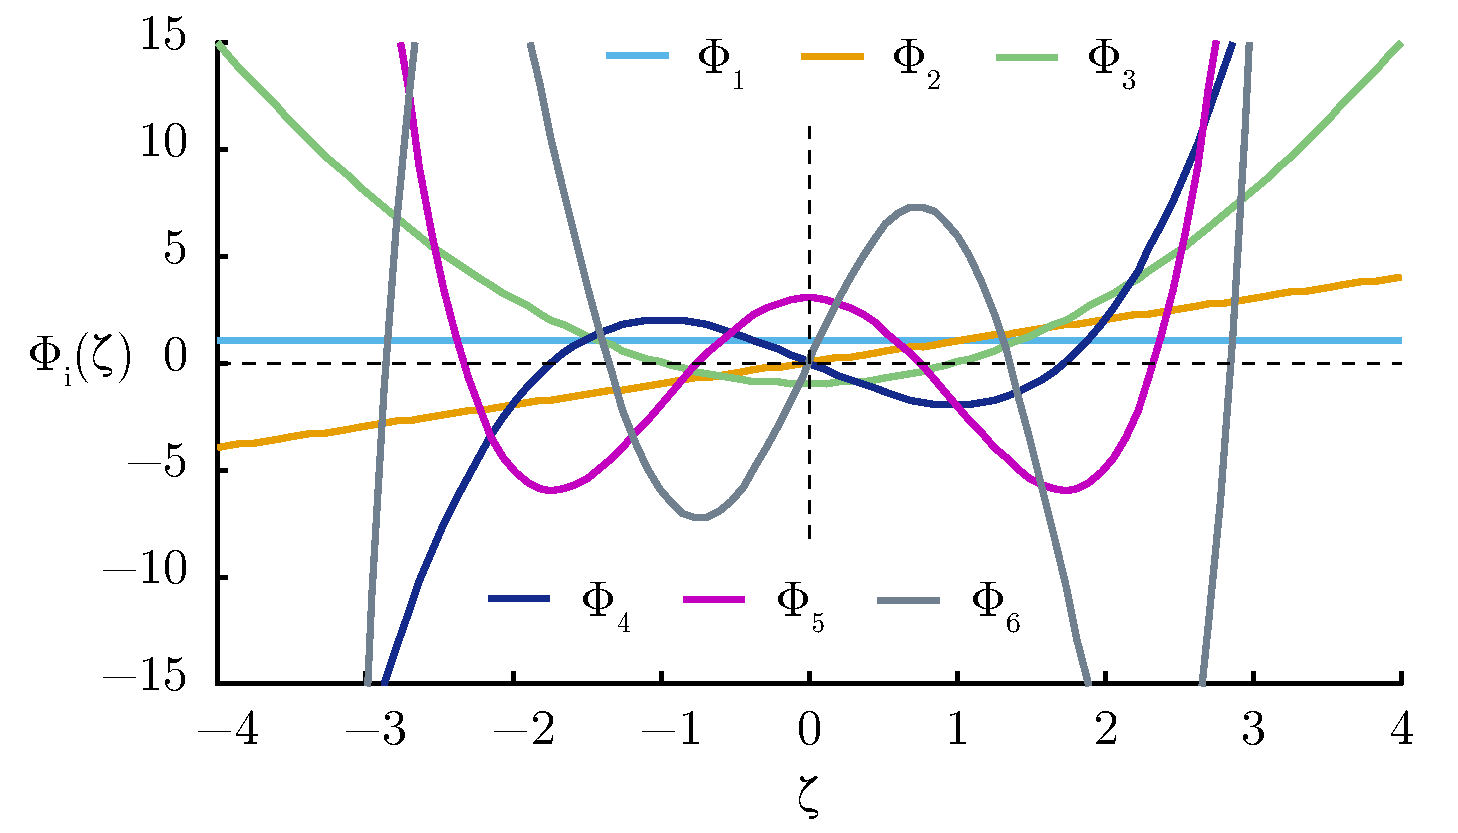
\includegraphics[width=0.9\columnwidth]{include/assets/hermite.pdf}
  }
  \vspace{-1.0em}
  \caption{The first six polynomials of the Hermite basis.}
  \vspace{-1.5em}
  \flabel{hermite}
\end{figure}

\subsubsection{Polynomial basis}
The first step towards a polynomial expansion is the choice of a suitable polynomial basis $\{ \pcb_i(\vz) \}_{i = 1}^\infty$, which is typically made based on the Askey scheme of orthogonal polynomials \cite{xiu2010}.
The step is crucial as the rate of convergence of PC expansions closely depends on it.
Although there are no strict rules that guarantee the optimal choice \cite{maitre2010, knio2006}, there are best practices saying that one should be guided by the probability distributions of the (independent) random variables that drive the stochastic system at hand (see \aref{polynomial-chaos}).
In our case, these variables are $\vZ(\o)$.
\tref{askey} displays several examples of such paired probability distributions and polynomial bases.
For instance, when a random variable follows a beta distribution, the Jacobi basis is worth being tried first; on the other hand, the Hermite basis is preferable for Gaussian distributions.
In order to give a better intuition of what such a basis may look like, \fref{hermite} plots the first six polynomials $\{ \pcb_i(\z) \}_{i = 1}^6$, $\z \in \real$, of the Hermite basis in one dimension.
In multiple dimensions, which is the case with the $\nvars$-dimensional random variable $\vZ(\o)$, several (possibly different) univariate bases are to be combined together to produce a single $\nvars$-variate polynomial basis $\{ \pcb_i(\vz) \}_{i = 1}^\infty$, $\vz \in \real^\nvars$ (see \cite{xiu2010, maitre2010}).

\subsubsection{Recurrence of polynomial expansions}
Having an appropriate basis chosen, we apply the PC expansion formalism to the power term in \eref{recurrence} and truncate the resulting infinite series in order to make it feasible for practical implementations.
Such an expansion is defined as
\begin{equation} \elabel{pc-expansion}
  \oPC{\nvars}{\pcorder}{\vP_k(\o)} := \sum_{i = 1}^{\pcterms} \pcc{\vP}_{ki} \; \pcb_i(\vZ(\o))
\end{equation}
where $\{ \pcb_i(\vz) \}_{i = 1}^{\pcterms}$, $\vz \in \real^\nvars$, is the truncated basis with $\pcterms$ polynomial terms of $\nvars$ variables, and $\pcc{\vP}_{ki} \in \real^\nprocs$ are the coefficients of the expansion.
The latter are computed using spectral projections as it is described in \sref{pc-coefficients}.
$\pcorder$ denotes the order of the expansion, which determines the maximal degree of the $\nvars$-variate polynomials involved in the expansion; hence, $\pcorder$ also determines the resulting accuracy.
The total number of the PC coefficients, $\pcterms$, is given by the following expression, which corresponds to the total-order polynomial space \cite{eldred2008, beck2011}:
\begin{equation} \elabel{pc-terms}
  \pcterms = { \pcorder + \nvars \choose \nvars } = \frac{(\pcorder + \nvars)!}{\pcorder! \, \nvars!}.
\end{equation}

It can be seen in \eref{recurrence} that, due to the linearity of the operations involved in the recurrence, $\vX_k(\o)$ retains the same polynomial structure as $\vP_k(\o)$. Therefore, using \eref{pc-expansion}, \eref{recurrence} is rewritten as follows, for $k = 1, \dotsc, \nsteps$:
\begin{equation} \elabel{expanded-recurrence}
  \oPC{\nvars}{\pcorder}{\vX_k(\o)} = \mCF_k \: \oPC{\nvars}{\pcorder}{\vX_{k-1}(\o)} + \mCS_k \: \oPC{\nvars}{\pcorder}{\vP_k(\o)}.
\end{equation}
Thus, there are two PC expansions for two concurrent stochastic processes with the same basis but different coefficients.

Using the definition in \eref{pc-expansion}, \eref{expanded-recurrence} can be explicitly written as follows:
\[
  \sum_{i = 1}^{\pcterms} \pcc{\vX}_{ki} \: \pcb_i(\vZ(\o)) = \sum_{i = 1}^{\pcterms} \left( \mCF_k \: \pcc{\vX}_{(k - 1)i} + \mCS_k \: \pcc{\vP}_{ki} \right) \pcb_i(\vZ(\o)).
\]
Multiplying the above equation by each polynomial from the basis and making use of the orthogonality property (given in \eref{orthogonality} in \aref{polynomial-chaos}), we obtain the following recurrence:
\begin{equation} \elabel{pc-recurrence}
  \pcc{\vX}_{ki} = \mCF_k \: \pcc{\vX}_{(k - 1)i} + \mCS_k \: \pcc{\vP}_{ki}
\end{equation}
where $k = 1, \dotsc, \nsteps$ and $i = 1, \dotsc, \pcterms$. Finally, \eref{fourier-output} and \eref{pc-recurrence} are combined together to compute the coefficients of the PC expansion of the temperature vector $\vTO_k(\o)$.

\subsubsection{Expansion coefficients} \slabel{pc-coefficients}
The general formula of a truncated PC expansion applied to the power term in \eref{recurrence} is given in \eref{pc-expansion}.
Let us now find the coefficients of this expansion, $\pcc{\vP}_{ki}$, which will be propagated to temperature (using \eref{pc-recurrence} and \eref{fourier-output}).
To this end, a spectral projection of the stochastic quantity being expanded, \ie, $\vP_k(\o)$, is to be performed onto the space spanned by $\{ \pcb_i(\vZ(\o)) \}_{i = 1}^{\pcterms}$, where $\pcterms$ is the number of polynomials in the truncated basis.
This means that we need to compute inner products of \eref{power-model} with each polynomial from the basis as
\[
  \oInner{\vP_k(\o)}{\pcb_i(\vZ(\o))} = \oInner{\sum_{j=1}^{\pcterms} \pcc{\vP}_{kj} \: \pcb_j(\vZ(\o))}{\pcb_i(\vZ(\o))}
\]
where $\oInner{\cdot}{\cdot}$ stands for the inner product (see \aref{polynomial-chaos} for a definition), $i = 1, \dotsc, \pcterms$, and $k = 1, \dotsc, \nsteps$. Making use of the orthogonality property of the basis, we obtain
\begin{equation} \elabel{pc-coefficients}
  \pcc{\vP}_{ki} = \frac{1}{\pcn_i} \oInner{\vP_k(\o)}{\pcb_i(\vZ(\o))}.
\end{equation}
In general, the inner product in \eref{pc-coefficients}, given in \eref{inner-product} in \aref{polynomial-chaos}, should be evaluated numerically.
This task is independent from the development in this section and, therefore, is discussed separately in \aref{gauss-quadrature}.
It is worth being mentioned that, since $\vP(\o)$ depends on temperature (see \sref{power-model}), at each step of the iterative process in \eref{pc-recurrence}, the computation of $\pcc{\vP}_{ki}$ should be done with respect to the PC expansion of the temperature vector $\vTO_{k - 1}(\o)$.

\subsubsection{Computational challenges} \slabel{computational-challenges}
From the development above, it is important to note that the theory of PC expansions suffers from the so-called curse of dimensionality \cite{xiu2010, maitre2010, eldred2008}.
\eref{pc-terms} together with \eref{pc-coefficients} reveal this problem: when the number of stochastic dimensions increases, the number of polynomial terms as well as the complexity of the corresponding coefficients exhibit a growth, which is exponential without special treatments.
The problem does not have a general solution and is one of the central topics of many ongoing studies.
In this paper, we mitigate this issue by: (a) keeping the number of stochastic dimensions low using the KL decomposition as we shall see in \sref{ie-uncertain-parameters} and (b) utilizing efficient integration techniques as discussed in \aref{gauss-quadrature}.
\begin{table}[b]
  \vspace{-5pt}
  \centering
  \caption{Probability distributions and polynomial bases.}
  \begin{tabular*}{0.95\linewidth}{llc}
    \toprule
    Distribution & Polynomial basis & Weight function \\
    \midrule
    Gaussian & Hermite & $e^{{-\z^2}/{2}}$ \\
    Uniform & Legendre & $1$ \\
    Beta & Jacobi & $(1 - \z)^\alpha (1 + \z)^\beta$ \\
    Exponential & Laguerre & $e^{-\z}$ \\
    Gamma & Generalized Laguerre & $\z^\alpha e^{-\z}$ \\
    \bottomrule
  \end{tabular*}
  \tlabel{askey}
\end{table}


To summarize, let us recall the stochastic recurrence in \eref{recurrence} where, in the presence of correlations, an arbitrary functional $\vP_k(\omega)$ of the uncertain parameters $\vU(\o)$ and random temperature $\vTO_k(\o)$ (see \sref{power-model}) needs to be evaluated and combined with another random vector, $\vX_k(\omega)$.
Now the recurrence in \eref{recurrence} has been replaced with a purely deterministic recurrence in \eref{pc-recurrence} that involves only linear operations.
Thus, the performed spectral decompositions have effectively substituted the heavy thermal system in \eref{fourier-system} with a light polynomial surrogate defined by a set of basis functions $\{ \pcb_i(\vz) \}_{i = 1}^\pcterms$ and the corresponding sets of coefficients, namely, $\{ \pcc{\vP}_{ki} \}_{i = 1}^\pcterms$ for power and $\{ \pcc{\vTO}_{ki} \}_{i = 1}^\pcterms$ for temperature, where $k$ traverses the $\nsteps$ intervals of the considered time span.
Consequently, the output of the proposed PTA framework constitutes two stochastic profiles: the power and temperature profiles denoted by $\profileP{\o}$ and $\profileT{\o}$, respectively, which are ready to be analyzed.
